\chapter[Időlépéses program verifikálása]{Időlépéses módszereket alkalmazó program verifikálása}\label{chap: lin+nemlin verif.}

{\ }

A következőkben a \ref{chap: lin+nemlin progi}. fejezetben ismertetett lineáris  és a nemlineáris megoldó programok verifikálását végzem el szakirodalmi példákkal. A példák mindkét program esetében  Chopra könyvében \cite{chopra}  találhatók. A lineáris megoldó programban a 16.1 példát, a nemlineáris megoldóban pedig a 16.4 feladatot számoltam.


\section{A lineáris időlépéses megoldó program verifikálása gerjesztett rezgésre}\label{sec:linver}

{\ } 

A lineáris megoldó program verifikálását Chopra könyvének \cite{chopra} 16.1 példája alapján végeztem.   A könyvben az angolszász mértékegységek használatosak, így a verifikálás során a könnyebb átláthatóság érdekében én is ezeket használtam. A nehézségi gyorsulást mindenhol $386 in./sec^2$ értékkel számoltam. A feladatban egy ötszintes épületet vetünk alá egy teljes periódus szinuszos talajgyorsulásnak, és ennek vizsgáljuk a válaszát Newmark módszerrel, lineáris gyorsulást feltételezve. A  gyorsulást az $\mathbf{\ddot{u}}_{g,0}\sin{2\pi{t}}$ függvény írja le, az amplitúdója  $\mathbf{\ddot{u}}_{g,0} = 0.5 g$ , periódusideje 1 sec. A támaszrezgéshez tartozó teher ez alapján számítható. Az egyes szintek tömege 100 kips/g, a szintenkénti merevség pedig 100 kips/in.; a csillapítási tényező minden módban 5\%. A feladatban a klasszikus modális csillapítással számolunk. A vizsgálat 2 sec-ig tart, az időlépések nagysága 0.1 sec. A szerkezet geometriája a \ref{fig:ex3-a} ábrán, a talajgyorsulások függvénye pedig a \ref{fig:ex3-a} grafikonon látható.



\begin{figure}%
\centering
\subfigure[][]{%
\label{fig:41-a}%
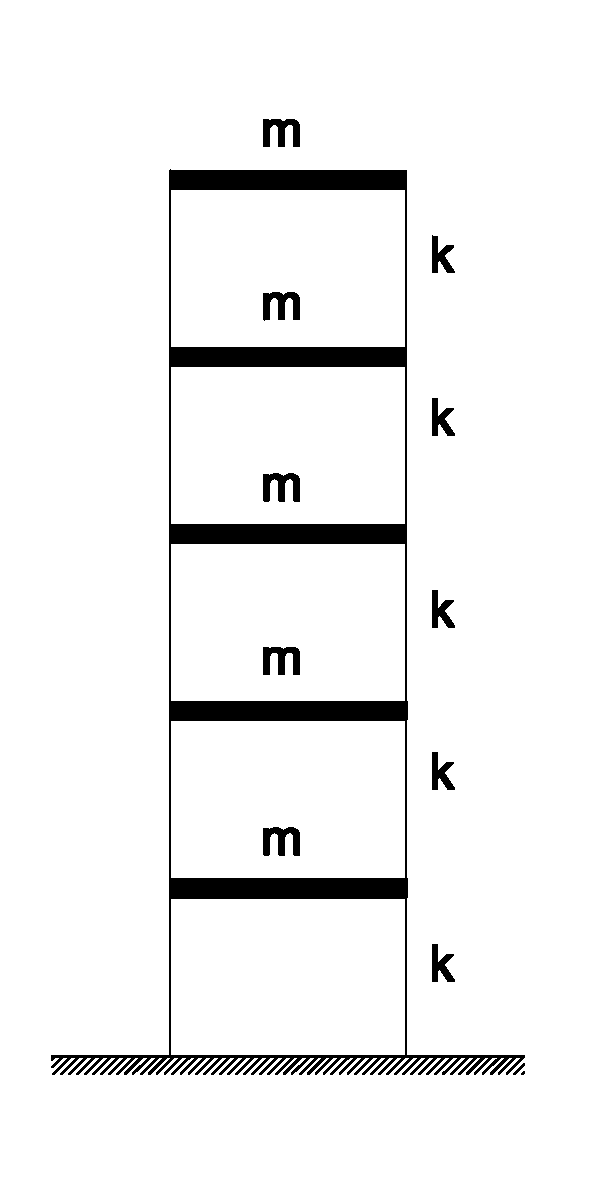
\includegraphics[width=0.25\textwidth]{otszintes_keret.pdf}}%
\hspace{8pt}%
\subfigure[][]{%
\label{fig:41-b}%
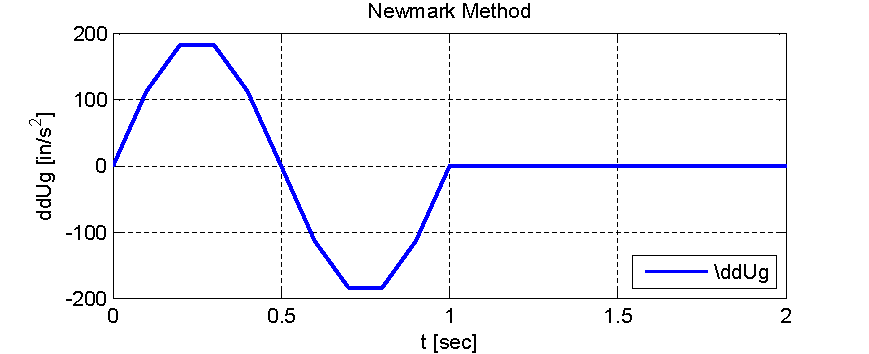
\includegraphics[width=0.7\textwidth]{41_ddUg.pdf}}%
\caption[A \cite{chopra} 16.1 feladatban vizsgált ötszintes keret és a  talajgyorsulás.]{\subref{fig:41-a} A \cite{chopra} 16.1 feladatban vizsgált ötszintes keret és \subref{fig:41-b}  a  talajgyorsulás}
 \label{fig:41}%
\end{figure}

A szerkezet analíziséhez modálanalízist és direkt integrálást együttesen alkalmaztunk. A számításhoz csak az első két módot használtuk, a többit elhanyagoltuk, így a rendszert kétszabadságfokúra redukáltuk. 

A rendszert leíró mátrixok a következők:
\begin{align*}
  & t_{max}  = 2 sec  & & \Delta{t} = 0,1 sec   & \\
  & \mathbf{M}  = 100\left[\begin{array}{rrrrr}  1 & 0 & 0 & 0 & 0  \\ 0 & 1 & 0 & 0 & 0 \\ 0 & 0 & 1 & 0 & 0 \\ 0 & 0 & 0 & 1 & 0 \\ 0 & 0 & 0 & 0 & 1  \end{array} \right] \frac{kips}{g}   &  & \mathbf{K} = 100 \left[\begin{array}{rrrrr} 2 & -1 & 0 & 0 & 0  \\ -1 & 2 & -1 & 0 & 0 \\ 0 & -1 &2 & -1 & 0 \\ 0 & 0 & -1 & 2 & -1 \\ 0 & 0 & 0 & -1 & 1 \end{array} \right]\frac{kips}{in.}  &  \\
  & \mathbf{C}_n  = \xi_n(2\mathbf{M}_n\omega_n)  &  & \xi = 0,05  & \\
  & \mathbf{q}_1  = -100\left[\begin{array}{c} 1 \\ 1 \\ 1 \\ 1 \\ 1 \end{array} \right]\mathbf{\ddot{u}}_{g}(t) & & \mathbf{\ddot{u}}_{g}(t) = \mathbf{\ddot{u}}_{g,0}\sin{2\pi{t}}  &  \\
  & \mathbf{u}(0)  = \left[\begin{array}{c} 0 \\ 0 \\ 0 \\ 0 \\ 0  \end{array} \right]  & & \mathbf{\dot{u}}(0) = \left[\begin{array}{c} 0 \\ 0 \\ 0 \\ 0 \\ 0 \end{array} \right] & 
  \end{align*}

A számítást Newmark módszerrel, lineáris gyorsulás feltételezésével végeztem. A módszerhez tartozó paraméterek értékei: $\gamma = \frac{1}{2}$ és $\beta = \frac{1}{6}$.

A szerkezetet bemeneti adatai az \verb|init_system.m| fájlban:
\lstinputlisting{"MATLAB/linear_system_41/init_system.m"}


A számított elmozdulások grafikonjai a \ref{fig:ex3} ábrán láthatók. A számítás az első modális szinten pontosnak tekinthető, mivel a lépésközök nagysága $\Delta{t} = 0,01 sec$, a sajátperiódusidő pedig $T_1 = 2\pi/5,592 = 1,12 sec$, tehát a lépésköz kisebb a természetes periódus tizedénél, teljesül az ökölszabály. Ugyanakkor a második modális szinten $\Delta{t}/T_2 = 0,16$ - ra adódik, ami nem felel meg a kritériumnak, ezért a második szint eredményei kevésbé pontosak. Ez a különbség megfigyelhető a  \ref{fig:ex3-a} és   \ref{fig:ex3-b} grafikonokon is. A modális elmozdulás görbéje az első szinten folytonosnak látszik, viszont a második szint modális elmozdulása inkább törött vonallal ábrázolható. 
 
\begin{figure}[h!b]%
\centering
\subfigure[][]{%
\label{fig:ex3-a}%
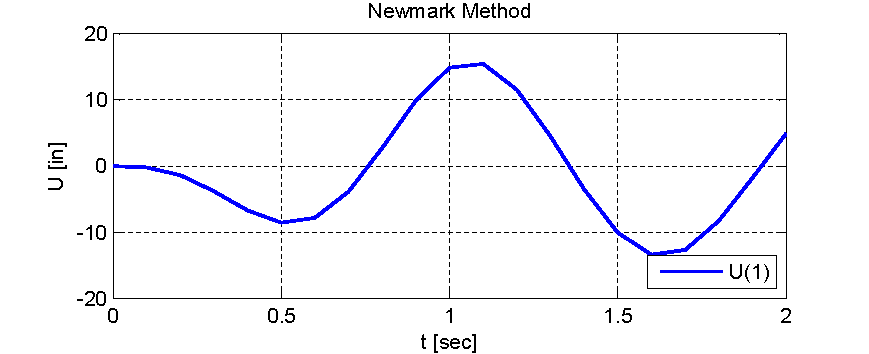
\includegraphics[width=0.75\textwidth]{41_U_1.pdf}}%
\\
\subfigure[][]{%
\label{fig:ex3-b}%
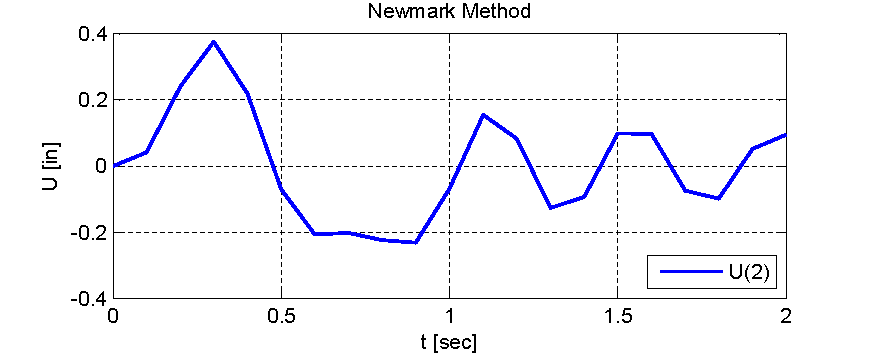
\includegraphics[width=0.75\textwidth]{41_U_2.pdf}}%
\\
\subfigure[][]{%
\label{fig:ex3-c}%
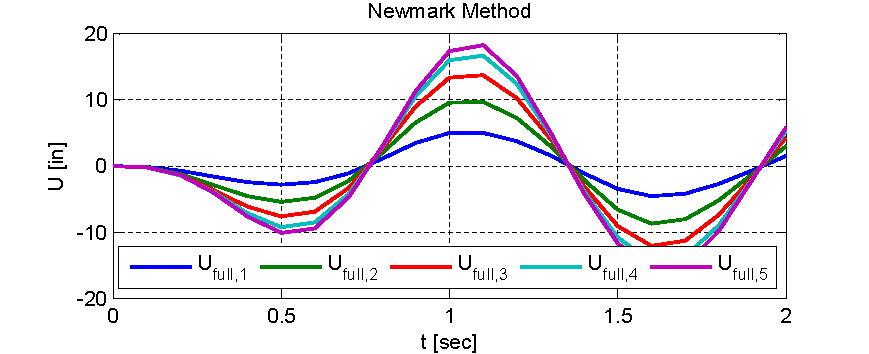
\includegraphics[width=0.75\textwidth]{41_U_full.pdf}}%
\caption[A \cite{chopra} 16.1 feladat eredményei a lineáris megoldó programmal.]{A \cite{chopra} 16.1 feladat eredményei a lineáris megoldó programmal:
\subref{fig:ex3-a} és \subref{fig:ex3-b}  modális elmozdulások;
\subref{fig:ex3-c} elmozdulások.}%
\label{fig:ex3}%
\end{figure}

A lineáris megoldó program számításainak eredményei négy tizedesjegy pontosan megegyeznek a könyvben közzétett eredményekkel. A számítás eredményei a \ref{161_table saját}, a könyvben ismertetett eredmények pedig a \ref{161_table} táblázatokban olvashatók. A \ref{161_table} referencia eredmények táblázatában a harmadik oszlop, ami modális elmozdulások  értékeit tartalmazza második szinten, feltehetőleg hibásan lett beírva, mivel ez megegyezik az első szint modális elmozdulásait mutató második oszloppal. Ettől a nyomdai hibától eltekintve a két táblázat megegyezik. A lineáris megoldó program verifikálása sikeresnek tekinthető.

\begin{table}[p]
\centering
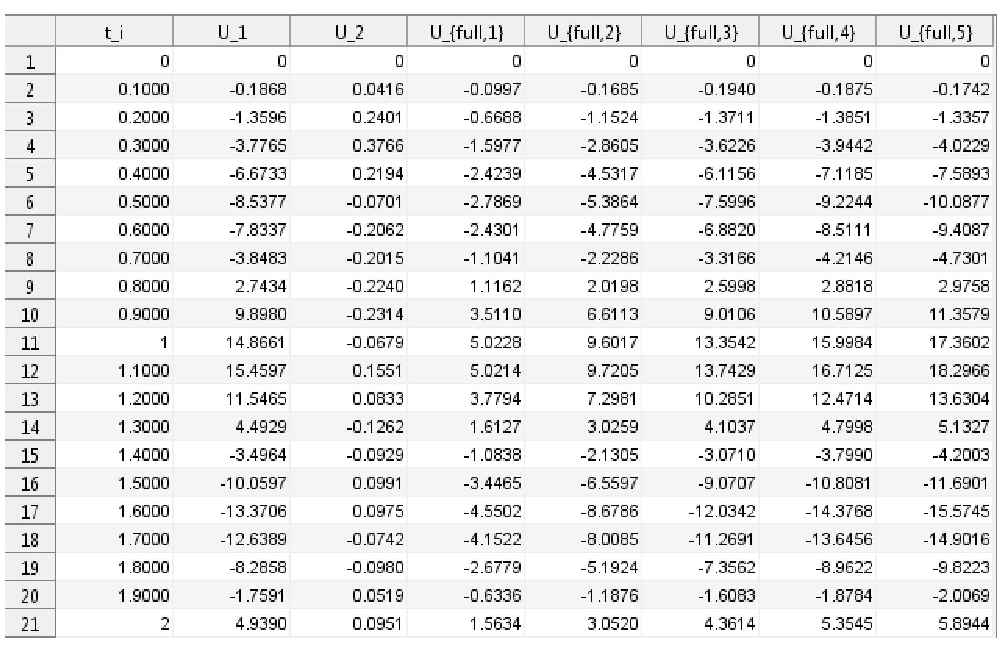
\includegraphics[width=\textwidth]{41_table.pdf}
\caption{A \cite{chopra} 16.1 példa megoldásai a lineáris megoldó programmal.}
\label{161_table saját}
\end{table}

\begin{table}[p]
\centering
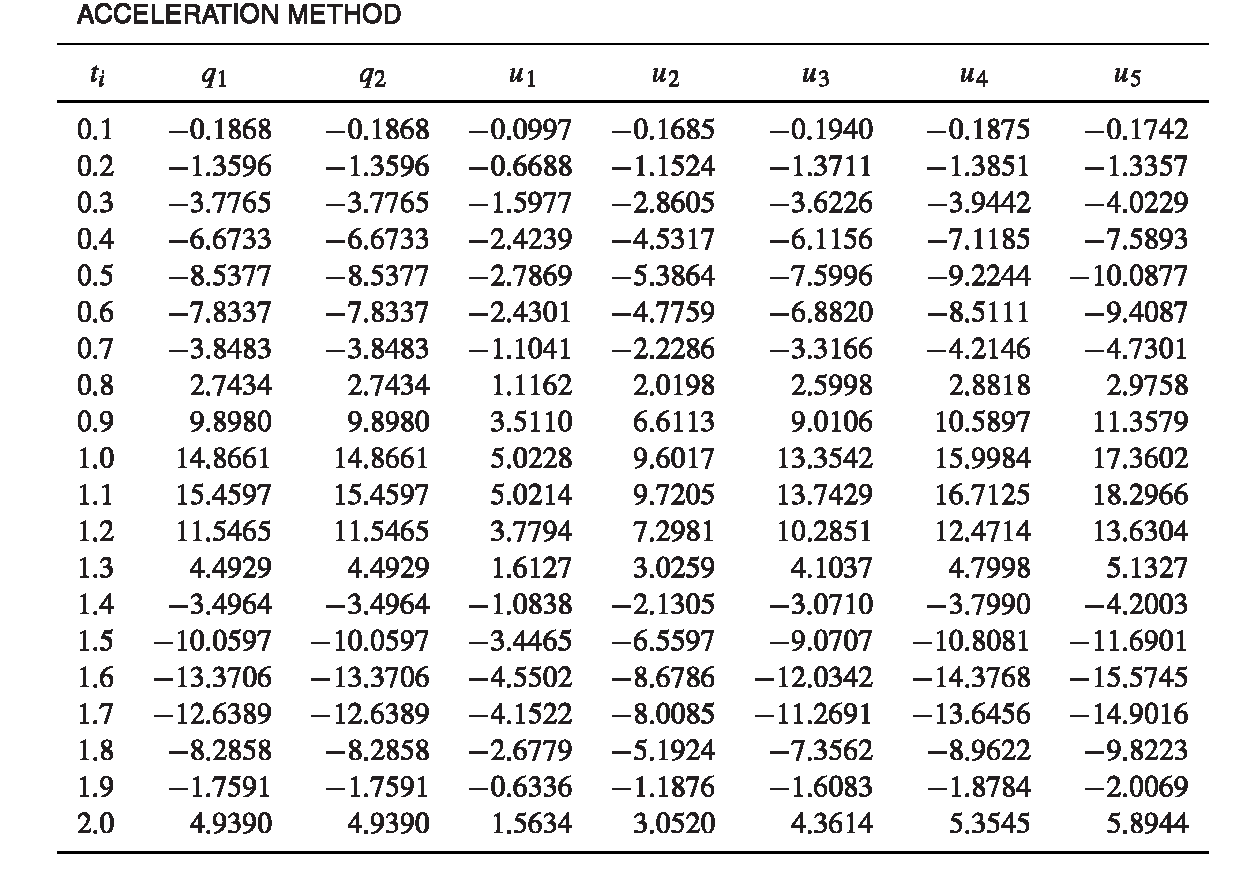
\includegraphics[trim = 0mm 0mm 0mm 7mm, clip, width=\textwidth]{41_chopra_table.pdf}
\caption{A \cite{chopra} 16.1 példa referencia  megoldásai.}
\label{161_table}
\end{table}




\newpage
\section{A nemlineáris időlépéses megoldó program verifikálása dinamikus problémára}

{\ }

A nemlineáris megoldó programot  Chopra könyvének \cite{chopra} 16.4 példája alapján verifikáltam.  Ebben a feladatban is az angolszász mértékegységekkel dolgoztam. A feladat szerint a könyv 16.1 példájából ismert  ötszintes keretet vizsgáljuk (\ref{fig:41-a} ábra), amire ugyanaz az 1 sec periódusidejű teljes szinuszhullám talajgyorsulás hat. A gyorsulás grafikonja a \ref{fig:41-b} ábrán látható. A mozgásegyenlet megoldását ezúttal a  konstans átlagos gyorsulást feltételező nemlineáris Newmark módszerrel oldottuk meg, az egyes időlépésekben kvázi-Newton-Raphson iterációval közelítve a megoldást. Az integrálási paraméterek értékei: $\gamma = \frac{1}{2}$ és $\beta = \frac{1}{4}$. 

A szerkezet anyagmodellje ezúttal a könyv 16.2 példájában alkalmazott  bilineáris  anyagmodell, $k = 100 kips/in.$ kezdeti merevséggel és $\alpha = 0.05$ utólagos merevség csökkenéssel. A határnyíróerő $V_{jy} = 125 kips$. Az anyagmodell diagramja a \ref{fig:nemlinpassz amodell} ábrán látható. Az anyagmodell ismertetése a könyvben hiányos, nem derül ki, hogy a felkeményedést követő visszaterhelésnél hogyan viselkedik az anyagunk. Az ismert adatok alapján egy lineárisan rugalmas - lineárisan felkeményedő anyagmodellt alkalmaztam.

\begin{figure}[h!]
\centering
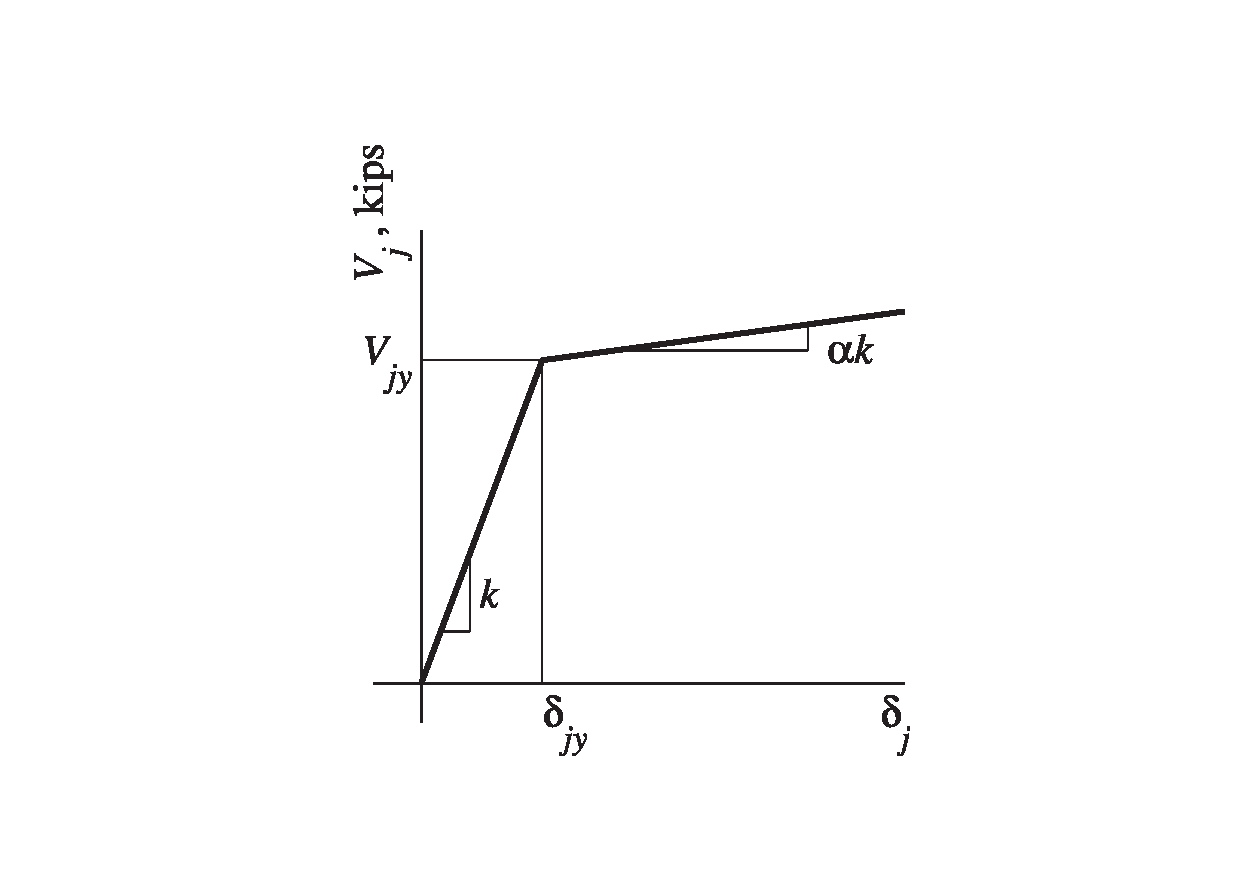
\includegraphics[width=0.75\textwidth]{bilin_amod.pdf}
\caption{A feladatban alkalmazott bilineáris anyagmodell \cite{chopra}}
\label{fig:nemlinpassz amodell}
\end{figure}

 A szerkezet tömeg- és merevségi mátrixát már korábban előállítottuk a \ref{sec:linver} pontban. A vizsgálat időlépése $0.1 sec$, a kezdeti feltételek zérus értékűek,  a csillapítási tényező minden módban 5\%.Ezúttal a teljes szerkezeten futtatjuk  a számításokat. A csillapítási mátrixot a példában  a modális csillapítási mátrixok szuperpozíciójával vettük figyelembe. Ez egy alternatív módszer a modális csillapítási tényezőkből előállított klasszikus csillapítási mátrix számítására. A csillapítási mátrixot a következő összefüggés alapján számítottuk:
\begin{equation*}
     \mathbf{C}  = \mathbf{M}(\sum_{n = 1}^{N}\frac{2\xi_n\omega_n}{M_n}v_nv^t_n)\mathbf{M}     
\end{equation*}

Az \verb|init_system.m| fájlban a szerkezet csillapítási mátrixának számítása és a visszatérítő erő számításához szükséges állandók: 

\lstinputlisting[firstline=44, lastline=58]{"MATLAB/nonlinear_system_42_keplekeny/init_system.m"}
\lstinputlisting[firstline=83, lastline=101]{"MATLAB/nonlinear_system_42_keplekeny/init_system.m"}

A visszatérítő erő és az érintőmerevség számítása a \verb|resisting_force.m| és \verb|tangent_stiffness.m| függvényekben:

\lstinputlisting{"MATLAB/nonlinear_system_42_keplekeny/resisting_force.m"}
\lstinputlisting{"MATLAB/nonlinear_system_42_keplekeny/tangent_stiffness.m"}

A \ref{fig:ize} ábrán az elmozdulások láthatók az idő függvényében. A   16.1 példa \ref{fig:ex3-c} ábrán látható elmozdulásaival összehasonlítva látható, hogy a képlékeny szerkezet ugyanazt  a terhelést a képlékenyedés megjelenését követően lassabban követi a lineáris szerkezetnél, viszont a maximális elmozdulások a képlékeny szerkezet esetében kisebbek. 

 
\begin{figure}[h!]
\centering
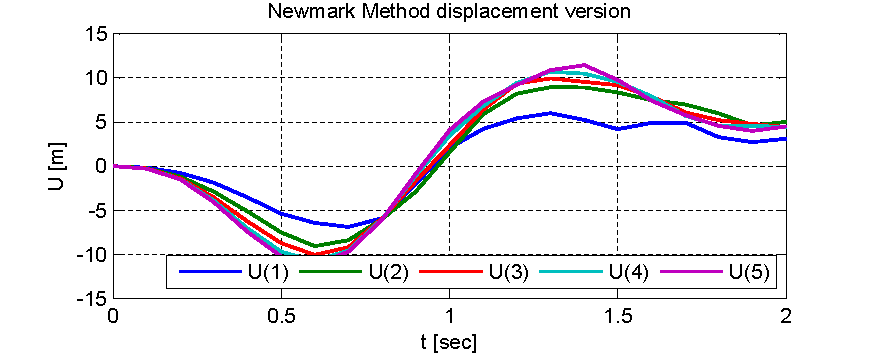
\includegraphics[width=\textwidth]{42_ufull.pdf}
\caption[A \cite{chopra} 16.4 feladat elmozdulásai a nemlineáris megoldó programmal.]{A \cite{chopra} 16.4 feladat elmozdulásai a nemlineáris megoldó programmal.}
\label{fig:ize}
\end{figure}


A \ref{164_table saját} és \ref{164_table} táblázatokban látható, hogy a nemlineáris megoldó programmal számított eredmények az első 6 sorban  négy tizedesjegy pontosan megegyeznek a könyvben ismertetett eredményekkel. Ezt követően azonban eltérések jelentkeznek a két táblázatban. Az első eltérés a 7. időpillanatban van, ez megegyezik a visszaterhelés kezdetével, vagyis  az különbségek a visszaterhelést követő számításokban jelennek meg. Ennek oka  az, hogy a példában az anyagmodell  hiányos leírása miatt  a könyv számításaihoz használt és az általam a nemlineáris programban alkalmazott anyagmodell eltérően veszi figyelembe a képlékenyedés utáni visszaterhelés hatását. Az első szakaszon számított megegyező eredmények miatt, és mert a második szakasz eredményeiben észlelt különbségek okát ismerjük, kijelenthetjük, hogy a nemlineáris megoldó program jól működik, a verifikálás sikeres.

\begin{table}[p]
\centering
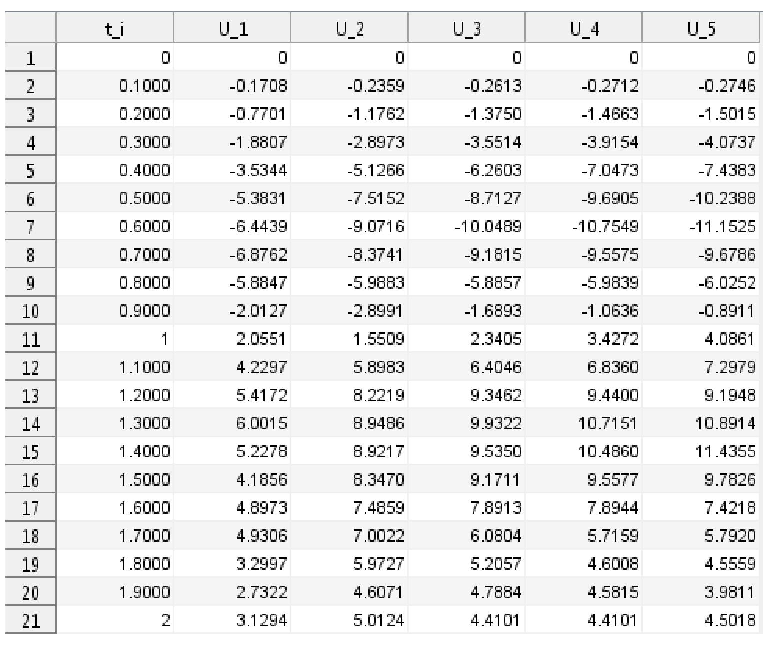
\includegraphics[width=0.8\textwidth]{42_table.pdf}
\caption{A \cite{chopra} 16.4 példa megoldásai a nemlineáris megoldó programmal.}
\label{164_table saját}
\end{table}

\begin{table}[p]
\centering
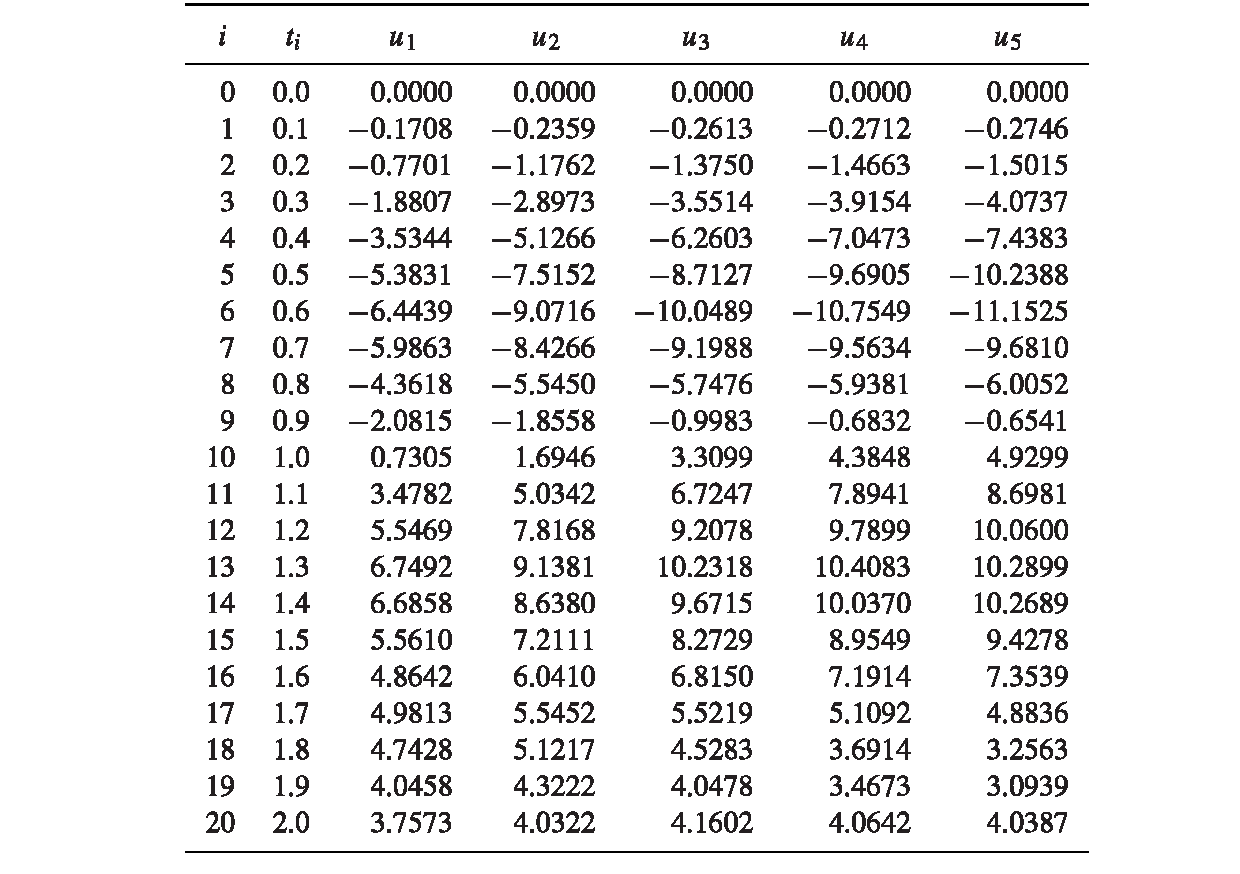
\includegraphics[width=\textwidth]{42_chopra_table.pdf}
\caption{A \cite{chopra} 16.4 példa referencia  megoldásai.}
\label{164_table}
\end{table}

